Electron scattering allows for finely tuned analysis of the nucleus. By manipulating the energy of the incoming electron and the kinematic variables accepted by the detectors used, experimenters can choose what aspect of the nucleus will be probed. This technique has been used to study the structure of the nucleus all the way down to the properties of the constituent quarks.

There are four kinematic regimes of electron scattering that can be explored: elastic, quasi-elastic, resonance, and deep inelastic scattering. Each of these regimes are defined by the kinematics and the underlying physical structure that they are sensitive to.

Elastic scattering occurs when the electron scatters coherently off of the nucleus. This occurs at low momentum and energy transfer. At these kinematics, the electron is sensitive to the size of the nucleus. The size of the nucleus is accessed by extracting nuclear ``form factors'' from the measured cross sections. From this we can learn about the charge distributions, magnetic moments, and charge radius of the nucleus.

Quasi-elastic scattering occurs at larger energy transfers when the electron scatters elastically off of the nucleon, rather than the nucleus. At these kinematics, the electron is sensitive to the form factors of the nucleon.

Resonance scattering occurs at even larger momentum and energy transfers. In this region, some of the energy is used to excite the nucleon into a higher energy state, called a resonance. A resonance is a short-lived particle. The resonance will quickly decay back into the nucleon and emit the excess energy as an additional particle. For example, $ep \rightarrow e\Delta^+ \rightarrow ep\pi^0$.

As we push the momentum and energy transfer further, we enter the Deep Inelastic Scattering (DIS) region. As $Q^2$ is increased into the transition region between resonance and DIS, the resonance peaks begin to smooth out. Here the electron becomes sensitive to the constituent parts of the nucleon. The wavelength of the exchanged photon is inversely proportional to $Q^2$. DIS scattering is of particular interest because the wavelength is sufficiently small enough to discern the parton structure. Through careful measurement, we can access the nuclear structure functions and the parton distributions in the the nucleons.\cite{HaM,PaN,NaPP}

The MARATHON experiment seeks to study the nuclear and nucleon structure functions, as well as nucleon parton distributions. The kinematics used are in the DIS region in order to facilitate this study. The remainder of this chapter will be focused on the DIS cross section and what we can learn from it.

%Inelastic scattering allows us to probe the internal structure of the nucleon. As $Q^2$ increases, baryon resonances begin to appear. As we push $Q^2$ even further past the resonance region, the wavelength of the virtual photon exchanged is short enough to discern the quark structure. This is known as the Deep Inelastic Scattering region.

\subsection{Deep Inelastic Scattering Cross Section}

Deep Inelastic Scattering, shown in Figure \ref{fig:feyn_dis}, involves a high energy electron scattering off of a nucleon. In the lowest order perturbation, a virtual photon is exchanged between the electron and nucleon. This momentum transfer then excites the nucleon into a hadronic final state. Though the final hadronic state is undetected, the detection of the scattered electron can yield insight into the interaction.

The reaction, for scattering off a proton, is written as:

\begin{equation*}
	e^- + P \rightarrow e^- + X
\end{equation*}

\begin{figure}
\begin{center}
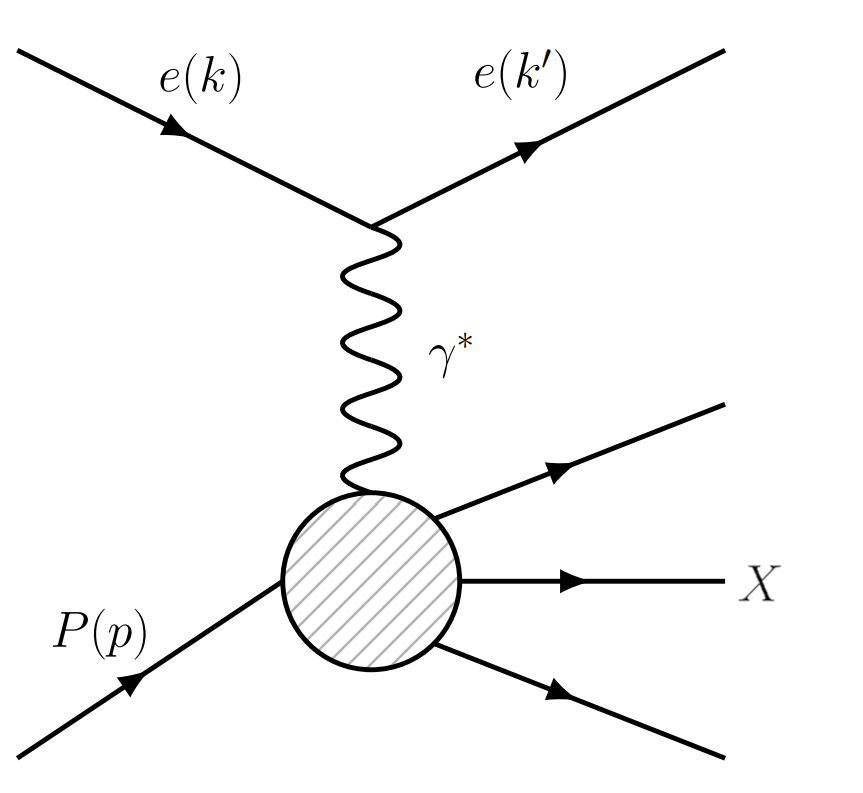
\includegraphics[width=.5\textwidth]{./scattering/fig/feyn_dis.png}
\caption{Feynman Diagram of Deep Inelastic Scattering}
\label{fig:feyn_dis}
\end{center}
\end{figure}

In this section, there will be many variables defined. For clarity, the meaning of these variable are defined in Table \ref{tab:var_def}. Mathematical definitions will follow as necessary.

\begin{table}
\center
\begin{tabular}{|l|l|}
\hline 
$Q^2$ & Negative of the 4-momentum transfer \\
$W^2$ & Square of the invariant mass of the final hadronic state \\
$E$ & Beam energy \\
$E^\prime$ & Scattered electron energy \\
$L_{\mu\nu}$ & Electron tensor \\
$W^{\mu\nu}$ & Symmetric hadronic tensor \\
$k$ & 4-momentum of the incident electron \\
$k^\prime$ & 4-momentum of the scattered electron \\
$p$ & 4-momentum of the target nucleon \\
$\theta$ & Scattered electron angle \\
$\nu$ & Energy difference between incoming and scattered electron \\
$M$ & Proton mass \\
$m$ & Electron mass \\
\hline
\end{tabular}
\caption{Variable definitions introduced in this section}
\label{tab:var_def}
\end{table}

The kinematics of scattering are typically defined by he Lorentz-invariant kinematic variables $Q^2$ and $W^2$, as well as the energy difference $\nu$. These variables are defined as:

\begin{equation}
	q^2 \equiv -Q^2 = \left(k-k^\prime\right)^2
\end{equation}

\begin{equation}
	W^2 = \left(p+q\right)^2
\end{equation}

\begin{equation}
	\nu = E-E^\prime
\end{equation}

Now it is useful to analyze in the laboratory rest frame and to note that MARATHON is a fixed target experiment. In this frame, the target is ``at rest'' (i.e. having a four-momentum of $\left(M,0\right)$). This leads to a simplification of $Q^2$ and $W^2$.

\begin{equation}
	Q^2 = 4EE^\prime\sin^2\frac{\theta}{2}
\end{equation}

\begin{equation}
	W^2 = M^2 + 2M\nu - Q^2
\end{equation}

Electron-nucleon scattering can be generally expressed as the following:

\begin{equation}
	\frac{d^2\sigma}{d\Omega dE^\prime} = \frac{\alpha^2}{Q^4}\frac{E^\prime}{E} L_{\mu\nu}W^{\mu\nu}
\end{equation}

%Here we define $Q^2$ as the 4-momentum transfer, $E$ as the beam energy, $E^\prime$ as the scattered electron energy, $L_{\mu\nu}$ as the electron tensor, and $W^{\mu\nu}$ as the symmetric hadronic tensor. The hadronic tensor is necessarily symmetric because the electron tensor is symmetric.

The electron tensor is expressed as:

%\begin{equation}
%	L_{\mu\nu} = \sum_{s,s^\prime}\overline{u}\left(k^\prime,s^\prime\right)\gamma_{\mu}u\left(k,s\right)\overline{u}\left(k,s\right)\gamma_{\nu}u\left(k^\prime,s^\prime\right)
%\end{equation}
%
%When evaluated, this yields:

\begin{equation}
	L_{\mu\nu} = 2\left(k^{\prime\mu}k^{\nu} + k^{\prime\nu}k^{\mu} - \left(k^{\prime}\cdot k - m^{2}\right)g^{\mu\nu}\right)
\end{equation}

The DIS hadronic tensor is expressed in terms of structure functions $W_1$ and $W_2$:

%\begin{equation}
%	W^{\mu\nu} = -W_{1}g^{\mu\nu} + \frac{W_2}{M^2}p^{\mu}p^{\nu} + \frac{W_4}{M^2}q^{\mu}q^{\nu} + \frac{W_5}{M^2}\left(p^{\mu}q^{\nu} + q^{\mu}p^{\nu}\right)
%\end{equation}
%
%Using current conservation at the hadronic vertex, two structure functions can be eliminated:

\begin{equation}
	W^{\mu\nu} = W_{1}\left(-g^{\mu\nu} + \frac{q^{\mu}q^{\nu}}{q^2}\right) + \frac{W_2}{M^2}\left(p^{\mu}-\frac{p\cdot q}{q^2}q^{\mu}\right)\left(p^{\nu}-\frac{p\cdot q}{q^2}q^{\nu}\right)
\end{equation}

Combining all of this, we arrive at the $ep$ DIS cross section in the laboratory frame:

\begin{equation}
	\left.\frac{d^2\sigma}{d\Omega dE^\prime}\right\rvert_{\mathrm{lab}} = \frac{\alpha^2}{4E^{2}\sin^{4}\frac{\theta}{2}} \left[W_{2}\cos^{2}\frac{\theta}{2} + 2W_{1}\sin^{2}\frac{\theta}{2}\right]
	\label{xs_inelastic}
\end{equation}

%%%%%%%%%%%%%%%%%%%%%%%%%%%%%%%%%%%%%%%%%%%%%%%%%%%%%%%%%%%%%%
%%%%%%%%%%%%%%%%%%%%%%%%%%%%%%%%%%%%%%%%%%%%%%%%%%%%%%%%%%%%%%
%Below here is old stuff that I'll pull from%%%%%%%%%%%%%%%%%%
%Don't keep this stuff%%%%%%%%%%%%%%%%%%%%%%%%%%%%%%%%%%%%%%%%
%%%%%%%%%%%%%%%%%%%%%%%%%%%%%%%%%%%%%%%%%%%%%%%%%%%%%%%%%%%%%%
%%%%%%%%%%%%%%%%%%%%%%%%%%%%%%%%%%%%%%%%%%%%%%%%%%%%%%%%%%%%%%

%Electron comes in, exchanges photon with nucleon. Boom.
%
%Deep inelastic scattering occurs at kinematics when the invariant mass, W, is greater than 2 GeV/$c^2$.
%
%At its most basic, Deep Inelastic Scattering (DIS) is the scattering of a lepton from a nucleon. The two participants exchange a virtual boson, the lepton scatters, and the nucleon is excited to a hadronic final state $X$ with higher mass.
%
%\begin{equation*}
%	\ell + N \rightarrow \ell^\prime + X
%\end{equation*}
%
%For the MARATHON experiment we will focus on electromagnetic DIS. In this case the lepton is charged and the exchanged virtual boson is a virtual photon. The JLab CEBAF accelerator provides an electron beam, so from here on the lepton will be written as an electron.
%
%\begin{equation*}
%	e^- + N \rightarrow e^- + X
%\end{equation*}
%
%\textbf{PUT DIS FEYNMAN DIAGRAM HERE}
%
%By interacting with a single nucleon, DIS is a powerful tool for studying nucleon structure. By looking at the DIS cross section, we can see how the nuclear structure functions readily present themselves.
%
%If we assume Lorentz invariance, \textbf{P} and \textbf{T} invariance, and conservation or lepton current, the cross section is
%
%\begin{equation}
%	\frac{d^2\sigma}{d\Omega dE^\prime} = \frac{\alpha^2}{Q^4}\frac{E^\prime}{E} L^{\left(s\right)^{\mu\nu}}W^{\left(s\right)}_{\mu\nu}
%\end{equation}
%
%where $Q^2$ is the 4-momentum transfer, $E$ is the beam energy, $E^\prime$ is the scattered electron energy, $L^{\left(s\right)^{\mu\nu}}$ is the lepton tensor, and $W^{\left(s\right)}_{\mu\nu}$ is the symmetric hadronic tensor.
%
%When written explicitly in the laboratory frame, we arrive at
%
%\textbf{DIS Cross Section}
%
%\begin{equation}
%	\sigma \equiv \frac{d^2\sigma}{d\Omega dE^\prime}\left(E,E^\prime,\theta\right) = \frac{4\alpha^2\left(E^\prime\right)}{Q^4}\cos^2\left(\frac{\theta}{2}\right)\left[\frac{F_2\left(\nu,Q^2\right)}{\nu}+\frac{2F_1\left(\nu,Q^2\right)}{M}\tan^2\left(\frac{\theta}{2}\right)\right]
%\end{equation}